\documentclass[10pt]{beamer}
\usetheme[
%%% option passed to the outer theme
%    progressstyle=fixedCircCnt,   % fixedCircCnt, movingCircCnt (moving is deault)
  ]{Feather}
  
% If you want to change the colors of the various elements in the theme, edit and uncomment the following lines

% Change the bar colors:
%\setbeamercolor{Feather}{fg=red!20,bg=red}

% Change the color of the structural elements:
%\setbeamercolor{structure}{fg=red}

% Change the frame title text color:
%\setbeamercolor{frametitle}{fg=blue}

% Change the normal text color background:
%\setbeamercolor{normal text}{fg=black,bg=gray!10}

%-------------------------------------------------------
% INCLUDE PACKAGES
%-------------------------------------------------------

% General
\usepackage[utf8]{inputenc}
\usepackage[portuguese]{babel}
\usepackage[T1]{fontenc}
\usepackage{helvet}

% Code syntax highlight
\usepackage{setspace}
\usepackage{color}
\usepackage{listings}

% Specify table cell length
\usepackage{array}

% Hyperlink reference
\usepackage{hyperref}

%-------------------------------------------------------
% DEFFINING AND REDEFINING COMMANDS
%-------------------------------------------------------

% colored hyperlinks
\newcommand{\chref}[2]{
  \href{#1}{{\usebeamercolor[bg]{Feather}#2}}
}

%-------------------------------------------------------
% Configure syntax highlight
%-------------------------------------------------------
\lstset{
  backgroundcolor=\color{white},
  breaklines=true,
  commentstyle=\color{green},
  extendedchars=true,
  frame=single,
  keepspaces=true,
  keywordstyle=\color{blue},
  language=Ruby,
  numbers=left,
  numbersep=10pt,
  numberstyle=\small\color{gray},
  rulecolor=\color{black},
  stringstyle=\color{blue},
  tabsize=2
}
%-------------------------------------------------------
% INFORMATION IN THE TITLE PAGE
%-------------------------------------------------------

% [] is optional - is placed on the bottom of the sidebar on every slide
% is placed on the title page
\title[] { 
\textbf{Princípios SOLID}
}

\subtitle[Princípios SOLID] {
}

\author[Seminário POO] {
Caio Costa Salgado \\
Leonardo Pereira Macedo \\
Rodrigo Siqueira Jordão
}

\institute[] {
Instituto de Matemática e Estatística \\
Universidade de São Paulo \\

% there must be an empty line above this line - otherwise some unwanted space
% is added between the university and the country (I do not know why;( )
}

\date{\today}

%-------------------------------------------------------
% THE BODY OF THE PRESENTATION
%-------------------------------------------------------

\begin{document}

%-------------------------------------------------------
% THE TITLEPAGE
%-------------------------------------------------------

{\1% % this is the name of the PDF file for the background
% the plain option removes the header from the title page, noframenumbering removes the numbering of this frame only
\begin{frame}[plain,noframenumbering] 
  \titlepage % call the title page information from above
\end{frame}
}

\begin{frame}{Sumário}{}
  \tableofcontents
\end{frame}

%=======================================================
\section{Introdução}
%=======================================================

\begin{frame}{Introdução}{Padrões e Antipadrões}

\begin{itemize}
  \item \textbf{Padrões de projeto}
  \begin{itemize}
    \item Solução reutilizável de um problema em design de \textit{software}
    \item Melhoram a qualidade e organização das classes
  \end{itemize}
  \pause
  \item \textbf{Antipadrões}
  \begin{itemize}
    \item Ineficientes, arriscados e contraprodutivos
    \item Podem ser identificados pelo \textbf{mau cheiro de projeto} que criam
  \end{itemize}
\end{itemize}

\begin{figure}[cheiroProjeto]
  
\includegraphics[width=0.45\textwidth]{images/codeSmell.jpg}
\end{figure}

\end{frame}

%-------------------------------------------------------

\begin{frame}{Princípios SOLID}{Introdução}
\begin{columns}

\begin{column}{0.7\textwidth}
  \begin{itemize}
    \item Acrônimo para 5 princípios de \textit{POO}
    \item Criado por Robert C. Martin \textit{(Uncle Bob)} por volta do ano 2000
    \item<2-> Diminui o acoplamento entre classes
    \item<2-> Separa as responsabilidades para melhorar o código da aplicação desenvolvida
  \end{itemize}
\end{column}

\begin{column}{0.25\textwidth}
  \begin{figure}[uncleBob]
    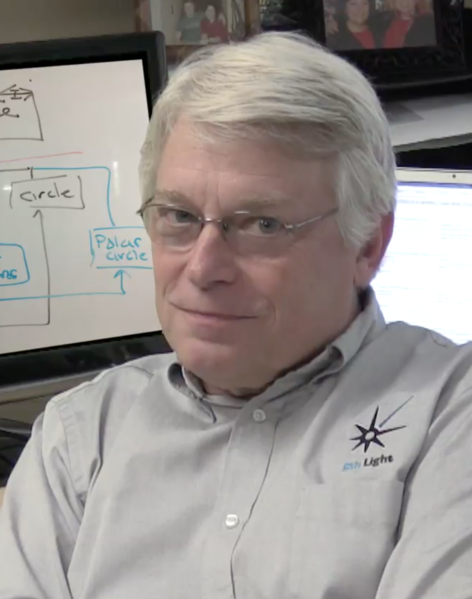
\includegraphics[width=1.2\textwidth]{images/uncleBob.png}
    % https://upload.wikimedia.org/wikipedia/commons/thumb/e/ee/Robert_Cecil_Martin.png/472px-Robert_Cecil_Martin.png
  \end{figure}
\end{column}

\end{columns}
\end{frame}

%-------------------------------------------------------

\begin{frame}{Acrônimo SOLID}{Introdução}

\begin{table}[H]
  \centering
  \setlength{\tabcolsep}{1pt}
  \begin{tabular}{cl}
    \Huge \textcolor{blue}{S} & \large ingle Responsibility \\
    \Huge \textcolor{blue}{O} & \large pen/Closed \\
    \Huge \textcolor{blue}{L} & \large iskov Substitution \\
    \Huge \textcolor{blue}{I} & \large njection of Dependencies \\
    \Huge \textcolor{blue}{D} & \large emeter Principle \\
  \end{tabular}
\end{table}

\end{frame}

%=======================================================
\section{Responsabilidade Única}
%=======================================================

\begin{frame}{\textbf{\textcolor{yellow}{S}OLID: Responsabilidade Única}}
	\begin{figure}[ht]
 		\centering
    	
\includegraphics[width=0.85\textwidth, keepaspectratio=true]{images/srp.jpg}
        % http://www.invitromagazine.gr/wp-content/uploads/2014/05/MASXALI2.jpg
	\end{figure}
\end{frame}

%-------------------------------------------------------

\begin{frame}{Responsabilidade Única}{Definição}

\begin{block}{PRU - Princípio de Responsabilidade Única}
Uma classe deve ter uma, e apenas uma, responsabilidade (isto é, apenas uma razão para mudar)
\end{block}

\begin{itemize}
  \item Uma responsabilidade pode ser descrita com 25 ou menos palavras
  \item Falta de \textbf{coesão} pode indicar uma violação do \textit{PRU}
\end{itemize}

\end{frame}

%-------------------------------------------------------

% fragile adicionado por causa do lstlisting
\begin{frame}[fragile]{Responsabilidade Única}{Exemplo}
\begin{columns}

\begin{column}{0.8\textwidth}
\begin{lstlisting}
class MasterClass
  def performInitialization ...; end
  def readFromFile          ...; end
  def writeToFile           ...; end
  def displayToScreen       ...; end
  def performCalculation    ...; end
  def validateInput         ...; end
end
\end{lstlisting}
\end{column}

\pause

\begin{column}{0.1\textwidth}
  \begin{figure}
    
\includegraphics[width=1.5\textwidth]{images/toxicSign.png}
    % http://cdn.mysitemyway.com/etc-mysitemyway/icons/legacy-previews/icons-256/yellow-road-sign-icons-signs/097002-yellow-road-sign-icon-signs-warning-poison1.png
  \end{figure}
\end{column}

\end{columns}

\textit{MasterClass} contém responsabilidades diversas e pouco relacionadas

\end{frame}

%-------------------------------------------------------

% 'fragile' adicionado por causa do lstlisting
\begin{frame}[fragile]{Responsabilidade Única}{Exemplo}

\lstset {
  basicstyle=\footnotesize
}

Solução: Separar em classes de acordo com a responsabilidade

\begin{lstlisting}
class FileInputOutput
  def readFromFile ...; end
  def writeToFile  ...; end
end
\end{lstlisting}

\begin{lstlisting}
class UserInputOutput
    def displayToScreen ...; end
    def validateInput   ...; end
end
\end{lstlisting}

\begin{lstlisting}
class Logic
    def performInitialization ...; end
    def performCalculation    ...; end
end
\end{lstlisting}

\end{frame}

%-------------------------------------------------------

\subsection{LCOM}
\begin{frame}{Responsabilidade Única}{LCOM}

\begin{itemize}
  \item \textbf{LCOM:} \textit{Lack of Cohesion of Methods}
  \item Analisa a coesão de uma classe, medindo se ela consiste em múltiplos "aglomerados"
  \item Duas variantes principais:
\end{itemize}

% TODO: Descobrir um jeito de dar quebra de linha automática na 3ª coluna
\begin{table}[H]
  \centering
  \begin{tabular}{|c|c| m{5cm} |} \hline
    \textbf{Variante} & \textbf{Pontuação} & \textbf{Interpretação} \\\hline
    Henderson-Sellers & \textbf{0} a \textbf{1} & Quanto mais próximo de 1, mais variáveis de instância são acessadas por apenas um método \\\hline
    LCOM-4 & \textbf{1} a \textbf{n} & Se n > 1, então n-1 responsabilidades podem ser extraídas para suas próprias classes \\\hline
  \end{tabular}
\end{table}

\end{frame}

%-------------------------------------------------------

\begin{frame}{Responsabilidade Única}{LCOM-4}

\begin{itemize}
  \item Dois métodos estão relacionados se:
  \begin{itemize}
    \item Acessam a mesma variável de instância/classe
    \item Um chama o outro
  \end{itemize}
  \uncover<2->{
    \item LCOM-4 conecta métodos relacionados em um grafo 
    \item Se o número \textbf{n} de grafos resultantes for maior que 1, pode-se dividir em classe em partes menores
  }
\end{itemize}

  \only<3>{
    \begin{figure}
      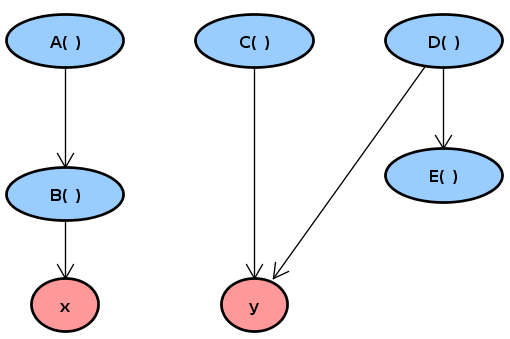
\includegraphics[width=0.55\textwidth]{images/LCOM4_a.png}
      \setbeamertemplate{caption}{\raggedright\insertcaption\par}
      \caption{Exemplo 1: LCOM-4 = 2}
    \end{figure}
  }

  \only<4>{
    \begin{figure}
      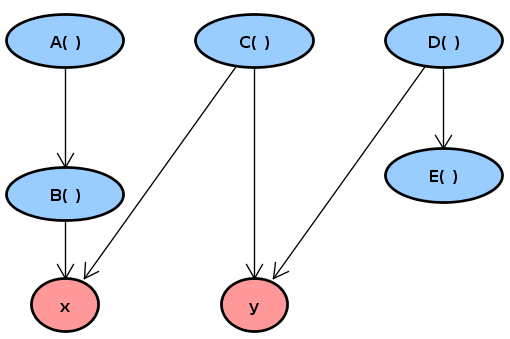
\includegraphics[width=0.55\textwidth]{images/LCOM4_b.png}
      \setbeamertemplate{caption}{\raggedright\insertcaption\par}
      \caption{Exemplo 2: LCOM-4 = 1}
    \end{figure}
  }

\end{frame}

%=======================================================
\section{Aberto/Fechado}
%=======================================================

\begin{frame}{\textbf{S\textcolor{yellow}{O}LID: Aberto/Fechado}}
	\begin{figure}[ht]
 		\centering
    	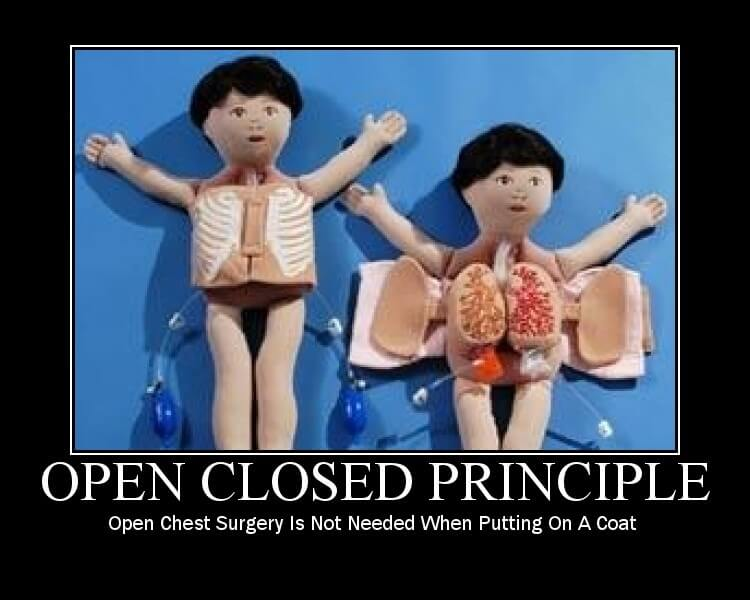
\includegraphics[width=0.85\textwidth, keepaspectratio=true]{images/openclosedprinciple.jpg}
	\end{figure}
\end{frame}

\begin{frame}{Aberto/Fechado}{Definição}

  \begin{block}{PAF - Princípio Aberto/Fechado}
  Uma classe deve ser aberta para extensão, mas fechada
  para modificação
  \end{block}

  \begin{itemize}
    \item Deseja-se estender o comportamento de classes
    sem modificar código existente na qual dependem
  \end{itemize}

\end{frame}

%-------------------------------------------------------

\begin{frame}[fragile]{Aberto/Fechado}{Exemplo}
\begin{columns}

\begin{column}{0.55\textwidth}
\lstset {
  basicstyle=\small
}

\begin{lstlisting}
class Report
  def output
    formatter = 
      case @format
      when :html
        HtmlFormatter.new(self)
      when :pdf
        PdfFormatter.new(self)
      end
  end
end
\end{lstlisting}
\end{column}

\pause

\begin{column}{0.59\textwidth}
  \begin{itemize}
    \item Cheiro de código \textit{Comando Case}...
    \pause
    \item \textbf{Cirurgia de Espingarda}: Adicionar um novo tipo de \textit{Formatter} exigirá mudanças em um ou mais métodos
    \begin{figure}
      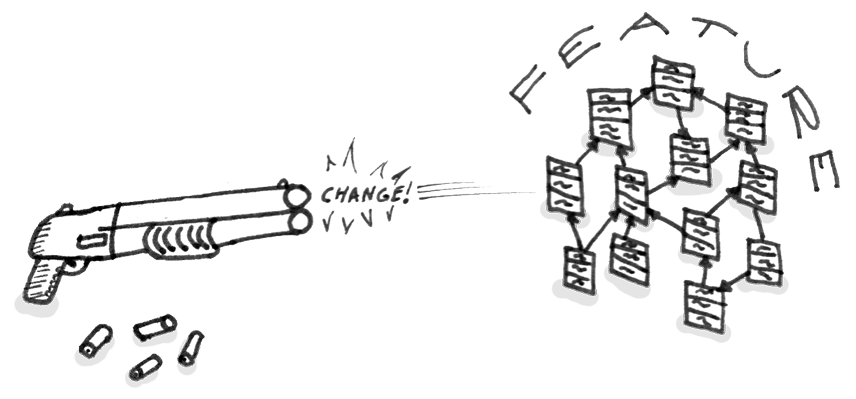
\includegraphics[width=0.85\textwidth]{images/shotgunSurgery.png}
    \end{figure}
  \end{itemize}
\end{column}

\end{columns}

\pause
\centering ~\\ Como resolver?
\pause \large \textbf{Padrões de projeto!}

\end{frame}

%-------------------------------------------------------

\subsection{Padrões de projeto úteis}
\begin{frame}[fragile]{Aberto/Fechado}{Solução com \textit{Fábrica Abstrata}}

\begin{lstlisting}
class Report
  def output
    formatter_class = 
      begin
        @format.to_s.classify.constantize
      rescue NameError
        # Handle "invalid formatter type"
      end
    formatter = formatter_class.send(:new, self)
  end
end
\end{lstlisting}

\begin{itemize}
  \item \textbf{@format} se refere a um símbolo (\textcolor{purple}{:pdf}, \textcolor{purple}{:html})
  \pause
  \item \textbf{\textit{Duck Typing:}} A partir do símbolo, adquirimos uma referência para a classe desejada e chamamos seu construtor
\end{itemize}

\end{frame}

%-------------------------------------------------------

\begin{frame}[fragile]{Aberto/Fechado}{Solução com \textit{Template}}

\begin{figure}
  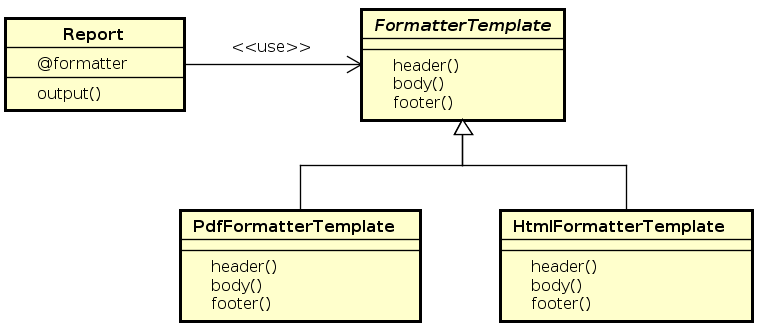
\includegraphics[width=1.0\textwidth]{images/templatePattern.png}
\end{figure}

\begin{itemize}
  \item Os passos (métodos) da tarefa (formatação) são os mesmos para todas as variantes de \textit{Formatter}
  \item Implementação dos métodos de cada subclasse podem divergir
\end{itemize}

\end{frame}

%-------------------------------------------------------

\begin{frame}[fragile]{Aberto/Fechado}{Solução com \textit{Strategy}}

\begin{figure}
  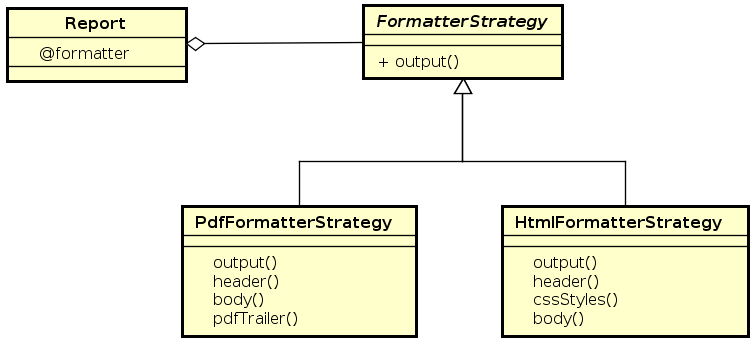
\includegraphics[width=1.0\textwidth]{images/strategyPattern.png}
\end{figure}

\begin{itemize}
  \item Usando \textbf{Strategy}, os passos podem ser diferentes em cada subclasse
\end{itemize}

\end{frame}

%-------------------------------------------------------

\subsection{Implementando novos comportamentos}
\begin{frame}{Aberto/Fechado}{Queremos Novos Comportamentos!}

\begin{itemize}
  \item E se quisermos adicionar um novo comportamento em uma classe existente? Por exemplo, arquivos PDF:
  \begin{itemize}
    \item Com/sem proteção de senha
    \item Com/sem uma marca d'água "rascunho"
  \end{itemize}
  \pause
  \item Uma possível ideia:
\end{itemize}

\setstretch{0}
\begin{columns}[T]

  \begin{column}{0.7\textwidth}
    \begin{figure}
      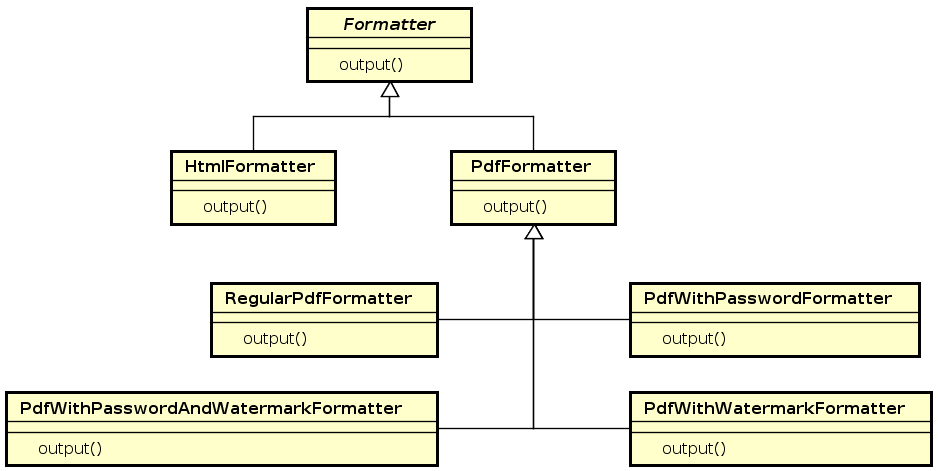
\includegraphics[width=1.3\textwidth]{images/badFormatterDesign.png}
    \end{figure}
  \end{column}

  \pause

  \begin{column}{0.3\textwidth}
    \begin{figure}
      
\includegraphics[width=0.35\textwidth]{images/toxicSign.png}
    \end{figure}
    \centering \large Não é \textbf{DRY}!
  \end{column}

\end{columns}

\end{frame}

%-------------------------------------------------------

\begin{frame}{Aberto/Fechado}{Padrão \textit{Decorator}}

\textbf{Padrão Decorator:} "Decoramos"\space a classe ao envolvê-la em uma versão melhorada, com mesma interface

\begin{figure}
  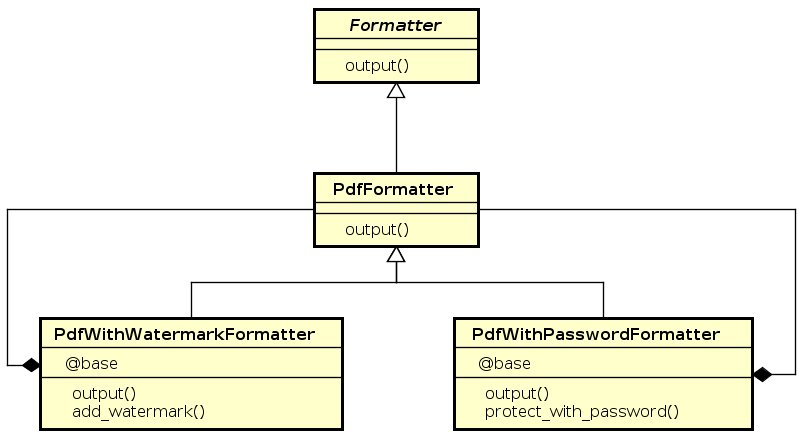
\includegraphics[width=1.0\textwidth]{images/decoratorPattern.png}
\end{figure}

\hfill \space \hfill \small \textcolor{blue}{\href{http://pastebin.com/u8aYdwEL}{\textit{Código fonte}}}

\end{frame}

%=======================================================
\section{Substituição de Liskov}
%=======================================================

\begin{frame}{\textbf{SO\textcolor{yellow}{L}ID: Substituição de Liskov}}
	\begin{figure}[ht]
 		\centering
    	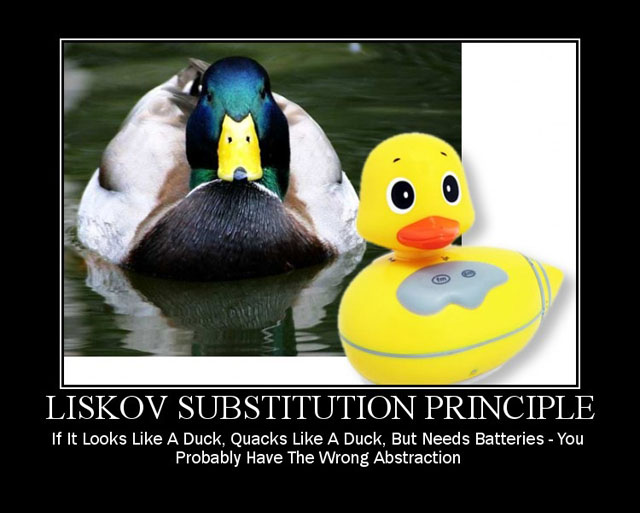
\includegraphics[width=0.85\textwidth, keepaspectratio=true]{images/LiskovSubstitution.jpg}
	\end{figure}
\end{frame}

%-------------------------------------------------------

\begin{frame}{Substituição de Liskov}{Definição}
  \begin{columns}[T]

    \begin{column}{.7\textwidth}
      \begin{block}{Princípio de Liskov}
      Um método projetado para trabalhar em um objeto de tipo T deve também trabalhar em um objeto de qualquer subtipo de T
      \end{block}
    \end{column}

    \hfill
    \begin{column}{.3\textwidth}
      \begin{figure}
        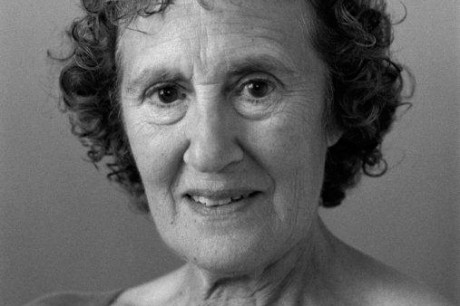
\includegraphics[width=1\textwidth]{images/Liskov.jpg}
      \end{figure}
    \end{column}
  \end{columns}

      \begin{itemize}
    	\item Herança é muito util para a reutilização de código, mas não é só por isso que ela deve ser usada
        \item A herança é um compartilhamento de implementação. Se a subclasse não ganha vantagem com a implementação herdada, talvez ela não devesse ser uma subclasse
  	\end{itemize}

\end{frame}

%-------------------------------------------------------
\begin{frame}[fragile]{Substituição de Liskov}{Exemplo}

\begin{lstlisting}
class Retangulo
  attr_accessor :largura, :altura, :canto_inf_esq
  def new(largura, altura, canto_inf_esq) ... ; end
  def area ... ; end
  def dobrar_altura_sobre_a_largura(dim)
    self.largura = 2*dim
    self.altura = dim
  end
end
class Quadrado < Retangulo
  attr_reader :largura, :altura, :lado
  def largura=(w)  ; @largura = @altura = w ; end
  def altura=(w) ; @largura = @altura = w ; end
  def lado=(w)   ; @largura = @altura = w ; end
end
\end{lstlisting}

\end{frame}
%-------------------------------------------------------
\begin{frame}{Substituição de Liskov}{Cheiro}
  \begin{block}{Mau cheiro}
    \begin{itemize}
      \item Modificação do funcionamento do método herdado
      \item Nesse caso, não faz sentido dobrar altura sobre a largura para um quadrado
      \item Método da superclasse jogado fora
    \end{itemize}
  \end{block}

  \begin{figure}
    
\includegraphics[width=0.2\textwidth]{images/toxicSign.png}
  \end{figure}

\end{frame}

%-------------------------------------------------------

\begin{frame}[fragile]{Substituição de Liskov}{Refatoração}
\begin{lstlisting}
class Quadrado
  attr_accessor :ret
  def initialize(:lado, :canto_inf_esq)
    @ret = Retangulo.new(lado, lado, canto_inf_esq)
  end
  
  def area
    ret.area
  end
  
  def lado=(s)
    rect.width = rect.height = s
  end
end
\end{lstlisting}
\pause
Trocando herança por composição: implementação é delegada, e não herdada
\end{frame}

%-------------------------------------------------------

\begin{frame}[fragile]{Substituição de Liskov}{Refatoração}
	\begin{block}{Delegação em Ruby: \textbf{Forwardable}}
	    Módulo em Ruby que implementa a delegação
	\end{block}
    \begin{lstlisting}
class Quadrado
  extend Forwardable
  def_delegators :@ret, :area, :perimetro, :rotacao

  def initialize(:lado, :canto_inf_esq)
    @ret = Retangulo.new(lado, lado, canto_inf_esq)
  end

  def lado=(s)
    @ret.largura = @ret.altura = s
  end
end
\end{lstlisting}
\end{frame}

%-------------------------------------------------------

\begin{frame}{Substituição de Liskov}
	\begin{block}{Resumo}
	Toda a implementação da super classe deve fazer sentido para as suas subclasses
	\end{block}
\end{frame}
%=======================================================
\section{Injeção de Dependência}
%=======================================================

\begin{frame}{\textbf{SOL\textcolor{yellow}{I}D: Injeção de Dependência}}
	\begin{figure}[ht]
 		\centering
    	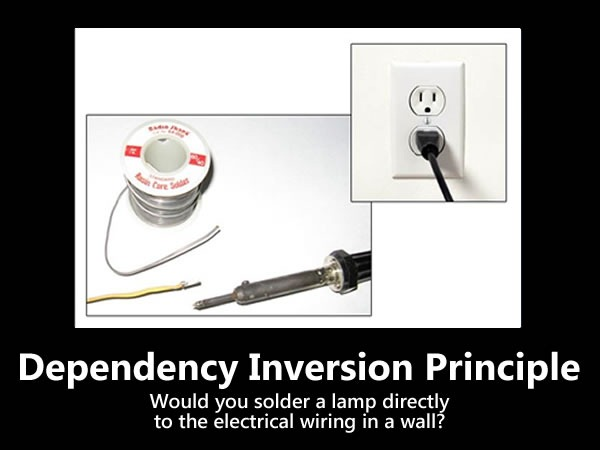
\includegraphics[width=0.85\textwidth, keepaspectratio=true]{images/dependency.jpg}
	\end{figure}
\end{frame}

%-------------------------------------------------------

\begin{frame}{Injeção de Dependêcia}{Definição}
  \begin{columns}[T]
    \begin{column}{.9\textwidth}
      \begin{block}{Injeção de dependência}
      \begin{itemize}
      \item Se duas classes dependem uma da outra, mas suas implementações podem mudar, seria bom para ambas dependerem de uma interface abstrata separada que seja "injetada"\space entre elas
      \pause
      \item O Princípio de Injeção de Dependência (PID) é a criação de uma interface com o objetivo de tratar a manipulação de objetos de forma correta em tempo de execução
      \end{itemize}
      \end{block}
    \end{column}
\end{columns}

\end{frame}

%-------------------------------------------------------

\begin{frame}[fragile]{Injeção de Dependêcia}{Exemplo}

\begin{lstlisting}
class EmailList
  attr_reader :mailer
  delegate :send_email, :to => :mailer
  def initialize 
    @mailer = MailerMonkey.new
  end
end
# in RottenPotatoes EmailListController:
def advertise_discount_for_movie
  moviegoers = Moviegoer.interested_in params[:movie_id]
  EmailList.new.send_email_to moviegoers
end
\end{lstlisting}

\end{frame}

%-------------------------------------------------------

\begin{frame}{Injeção de Dependêcia}{Exemplo}

\begin{itemize}
  \item Se quisermos adicionar novas maneiras para enviar mensagens, seria necessário modificar o funcionamento do \textit{controller}, adicionando condicionais
  \item Nesse caso, entra em ação o Princípio de Injeção de Dependência (PID)!
\end{itemize}

\end{frame}

%-------------------------------------------------------

\begin{frame}[fragile]{Injeção de Dependêcia}{Exemplo - Refatoração}
  \textbf{Controller}
  \begin{lstlisting}
def advertise_discount_for_movie
  moviegoers = Moviegoer.interested_in(params[:movie_id])
  EmailList.new(Config.emailer).send_email_to(moviegoers)
  end
end
\end{lstlisting}
\end{frame}

%-------------------------------------------------------

\begin{frame}[fragile]{Injeção de Dependêcia}{Exemplo - Refatoração}
  \textbf{Config Class}
  \begin{lstlisting}
class Config
  def self.emailer
    if email_disabled? then NullMailer else
      if has_amiko? then AmikoAdapter else MailerMonkey end
    end
  end
end
\end{lstlisting}
\end{frame}

%-------------------------------------------------------

\begin{frame}[fragile]{Injeção de Dependêcia}{Exemplo - Refatoração}
  \textbf{AmikoAdapter Class}
  \begin{lstlisting}
class AmikoAdapter
  def initialize ; @amiko = Amiko.new(...) ; end
  def send_email
    @amiko.authenticate(...)
    @amiko.send_message(...)
  end
end
\end{lstlisting}
\end{frame}

%-------------------------------------------------------

%\begin{frame}{Injeção de Dependêcia}{Exemplo - Refatoração}
%	\begin{figure}
%	\centering
%   \includegraphics[width=0.6\textwidth, keepaspectratio=true]{images/PID.png}
%	\end{figure}
%\end{frame}

%-------------------------------------------------------

\begin{frame}{Injeção de Dependêcia}{Padrões de Projeto}
	\textbf{PID pode ser uma aplicação de um padrão}
    \begin{itemize}
	\item \textit{Fachada}
    \item \textit{Fábrica abstrata:} Cria diferentes tipos de objetos com o mesmo objetivo  
    \item \textit{Adaptador:} Interface que modifica a interação com uma classe com o objetivo de padronizar o acesso (no nosso caso)
    \item \textit{Proxy:} Mesmo comportamento de outra classe, mas com tratamento para casos "estranhos"
	\end{itemize}
\end{frame}


%=======================================================
\section{Lei de Demeter}
%=======================================================

\begin{frame}{\textbf{SOLI\textcolor{yellow}{D}: Lei de Demeter}}
  \begin{figure}[ht]
    \centering
      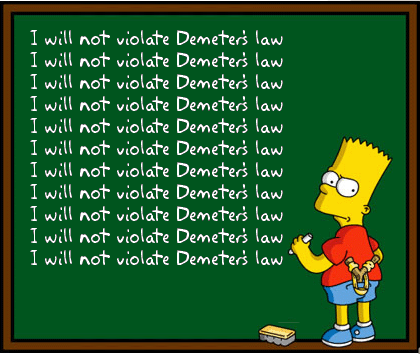
\includegraphics[width=0.65\textwidth, keepaspectratio=true]{images/simpson_demeterslaw.png}
  \end{figure}
\end{frame}

%-------------------------------------------------------

\begin{frame}{Lei de Demeter}{Definição}

  \begin{block}{Princípio de Demeter}
    Um método pode chamar outros métodos em sua própria classe e métodos nas classes de suas próprias variáveis de instância; todo o resto é tabu
    \end{block}

    \pause
    
    \begin{columns}[T]
      \begin{column}{.7\textwidth}
        \begin{block}{Conselhos...}
          Converse com seus amigos - Não fique íntimo de estranhos
        \end{block}

        \end{column}
        \hfill
        \begin{column}{.3\textwidth}
          \begin{figure}[ht]
          \centering
          
\includegraphics[width=0.8\textwidth, keepaspectratio=true]{images/strange.jpg}
            \end{figure}
        \end{column}
    \end{columns}
\end{frame}

%-------------------------------------------------------
\begin{frame}[fragile]{Lei de Demeter}{Demeter na Prática}
  \begin{block}{Seus parâmetros}
    Quando o seu método recebe parâmetros, ele pode chamar algum
    método fornecido por este parâmetro diretamente
  \end{block}

  \pause

\begin{lstlisting}
class JobPost
  def post_url(id)
    'http://www.kuniri.org/posts/#{id}'
  end
end
\end{lstlisting}

\end{frame}

\begin{frame}[fragile]{Lei de Demeter}{Demeter na Prática}
  \begin{block}{Qualquer objeto criado ou instanciado}
    Quando o seu método cria objetos locais, ele pode chamar
    métodos nos objetos locais
  \end{block}

  \pause

\begin{lstlisting}
class Mailer
  def prepare_emails(list)
    email_sanitizer = EmailSanitizer.new
    email_sanitizer.sanitize(list)
  end
end
\end{lstlisting}

\end{frame}

\begin{frame}[fragile]{Lei de Demeter}{Demeter na Prática}
  \begin{block}{Seu próprio componente de objeto}
    Seu método pode chamar métodos nos seus próprios campos diretamente 
    (mas não em campos do campo)
  \end{block}

  \pause

\begin{lstlisting}
class Mailer
  def initialize(email_sanitizer, list)
    @email_sanitizer = EmailSanitizer.new
    @list = list
  end

  def prepare_emails(list)
    @email_sanitizer.sanitize(list)
  end
end
\end{lstlisting}

\end{frame}

\begin{frame}[fragile]{Lei de Demeter}{Demeter na Prática}
  \begin{block}{A si mesmo}
    Seu método pode chamar outros métodos ou atributos na sua própria classe
    diretamente
  \end{block}

  \pause

\begin{lstlisting}
class Address
  attr_reader :city, :state
  
  def full_address
    "#{city}, #{state}"
  end
end
\end{lstlisting}

\end{frame}


\begin{frame}[fragile]{Lei de Demeter}{Exemplo}

\begin{lstlisting}

def sold_brand_email(order)
  @order = order
  mail(
   to: @order.line_items.last.brand.designer.email,
   subject: 'You sold a brand!')
end

\end{lstlisting}

  \pause

  \begin{figure}
    
\includegraphics[width=0.3\textwidth]{images/toxicSign.png}
  \end{figure}

\end{frame}

%-------------------------------------------------------

\begin{frame}[fragile]{Lei de Demeter}{Exemplo - Refatorando}

\begin{lstlisting}
class Mailer
  def send_mailer(order)
    mail(
     to: order.customer.email,
     subject: "Thanks for purchasing!")
  end
end
\end{lstlisting}

\end{frame}

\begin{frame}[fragile]{Lei de Demeter}{Exemplo - Aplicando a Lei de Demeter}

\begin{lstlisting}
class Mailer
  def send_mailer(order)
    customer_email = customer.email
    mail(
     to: order.customer_email,
     subject: "Thanks for purchasing!")
  end
end
\end{lstlisting}

\end{frame}

\begin{frame}[fragile]{Lei de Demeter}{Exemplo - Aplicando a Lei de Demeter}

\begin{lstlisting}
class Mailer
  def send_mailer(order)
    order.send_mailer
  end
end

class Order
  def send_mailer
    mail(
     to: customer.email,
     subject: "Thanks for purchasing!")
  end
end
\end{lstlisting}

\end{frame}

\begin{frame}{Bibliografia}{}
%-------------------------------------------------------
  \begin{itemize}
    \item Fox, A.; Patterson, D. \textit{Engineering Software as a Service}: An Agile Approach using Cloud Computing. Versão 1.1.1.
    \item http://rails-bestpractices.com/posts/2010/07/24/the-law-of-demeter/
    \item https://scotch.io/bar-talk/s-o-l-i-d-the-first-five-principles-of-object-oriented-design
    \item http://gespinosa.org/2015/law-of-demeter/
  \end{itemize}
\end{frame}

{\1
\begin{frame}[plain,noframenumbering]
  \finalpage{Obrigado pela atenção!}
\end{frame}}

\end{document}